\documentclass[11pt]{report}
\usepackage{graphicx}\graphicspath{D:\weather_station\report\final/}


\begin{document}
		\chapter*{\begin{center}
			PES INSTITUTE OF TECHNOLOGY SOUTH CAMPUS
			\end{center}}
			\begin{center}
				
\includegraphics{PES.jpg}\\
			\end{center}
			\textbf{{\LARGE \begin{center}
						DEPARTMENT OF COMPUTER SCIENCE AND ENGINEERING
					\end{center}}}
			
			{\LARGE \begin{center}
					WEATHER STATION USING RASPBERRY PI
				\end{center}}
			
			\begin{center}
				AKHIL CHOUHAN - 1PE15CS012
				
				AKSHAT TRIVEDI - 1PE15CS013
				
				CHEHAK NAYAR - 1PE15CS042
				
				DIVYAKSH SHUKLA - 1PE15CS051
			\end{center}

		\chapter*{\begin{center}
				Index
			\end{center}}
			
			\begin{flushleft}
				{\LARGE 	
					- Introduction\\
					
					- Hardware Requirements\\
					
					- Software Requirements\\
					
					- Expected Outcome\\
					
					- Result\\
					
					- Future Enhancements\\
				}	
			\end{flushleft}
	\chapter*{\begin{center}
			Introduction
		\end{center}}
		Weather station is a facility, either on land or sea, with instruments and equipment for measuring atmospheric conditions to provide information for weather forecasts and to study the weather and climate.It is a set of weather measuring instruments operated by a private individual, club, association, or even business (where obtaining and distributing weather data is not a part of the entity's business operation). The quality and number of instruments can vary widely, and placement of the instruments, so important to obtaining accurate, meaningful, and comparable data, can also be very variable.
		
		
		Today's personal weather stations also typically involve a digital console that provides readouts of the data being collected. These consoles may interface to a personal computer where data can be displayed, stored, and uploaded to Web sites or data ingestion/distribution systems.
		
		We aim o create a weather station to measure atmospheric conditions, humidity and acquire other weather related information.
		
		The project uses raspberry pi and integrates hardware allocated for specific tasks.The project measures the following : wind speed,temperature and humidity,rain,wind direction, pressure, level of pollution,sun lumens.Apart from this the weather station will also be capable of acquiring information for weather prediction from online sources.
		
					
	\chapter*{\begin{center}
			HARDWARE \\ REQUIREMENTS
		\end{center}}
	\chapter*{\begin{center}
			Raspberry Pi Model B+
		\end{center}}
	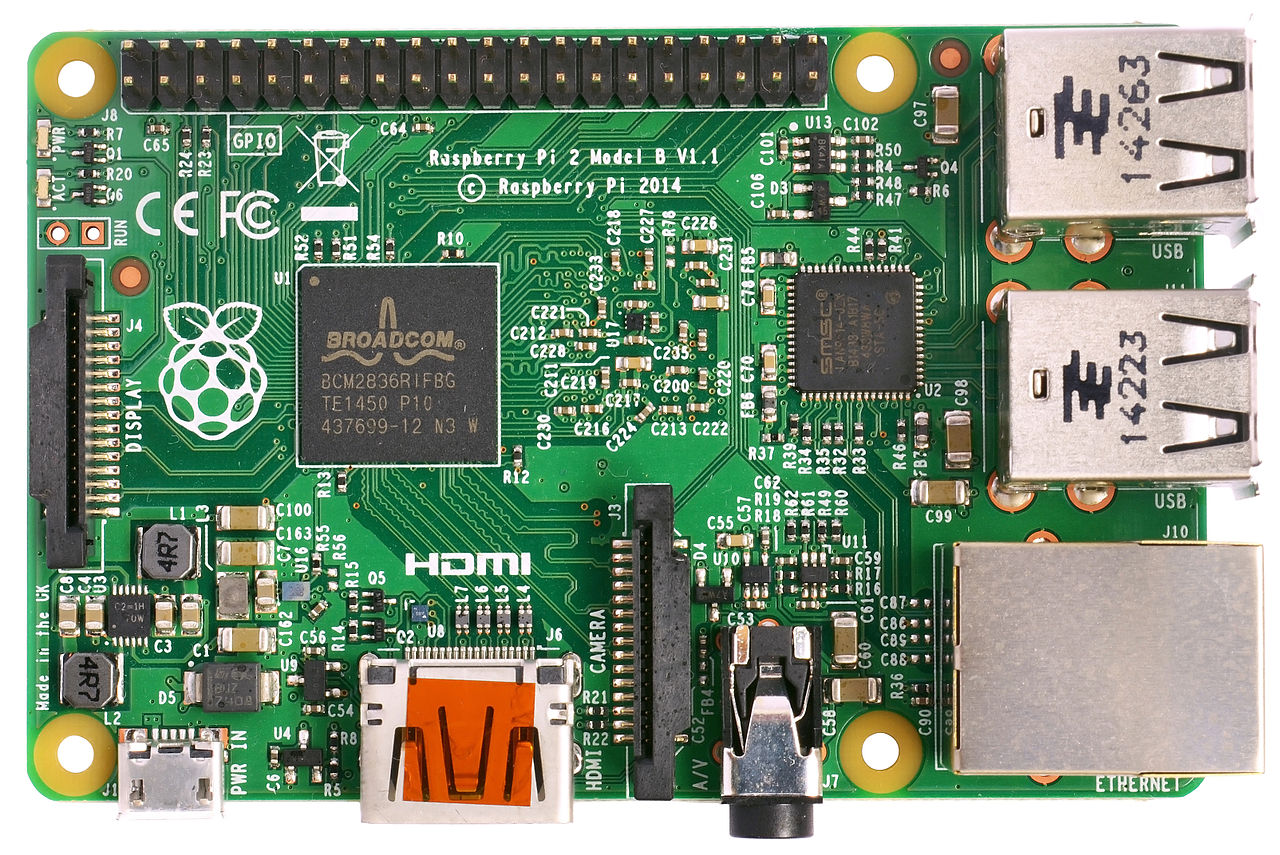
\includegraphics{raspi_b+.jpg}\\
	
	\textbf{Processor}
	
	BCM2837 - this is the Broadcom chip used in the Raspberry Pi 3. ARMv7 
	
	quad core cluster with a quad-core ARM Cortex A53 (ARMv8) cluster.\\\\
	
	\textbf{GPIO}
	
	General Purpose Input/Output pins on the Raspberry Pi\\
	
	OVERVIEW\\
	
	This page expands on the technical features of the GPIO pins available on 
	
	BCM2835 in general.\\
	
	GPIO pins can be configured as either general-purpose input, general-purpose 
	
	output or as one of up to 6 special alternate settings, the functions of which 
	
	are pin-dependent.
	
	There are 3 GPIO banks on BCM2835.
	
	Each of the 3 banks has its own VDD input pin. On Raspberry Pi, all GPIO 
	
	banks are supplied from 3.3V. Connection of a GPIO to a voltage higher 
	
	than 3.3V will likely destroy the GPIO block within the SoC.
	
	A selection of pins from Bank 0 is available on the P1 header on Raspberry 
	
	Pi.
	
	\chapter*{\begin{center}
			Sensors
		\end{center}}
	\underline{{\LARGE \textbf{MQ– 135} Air Quality Sensor}}\\
	
	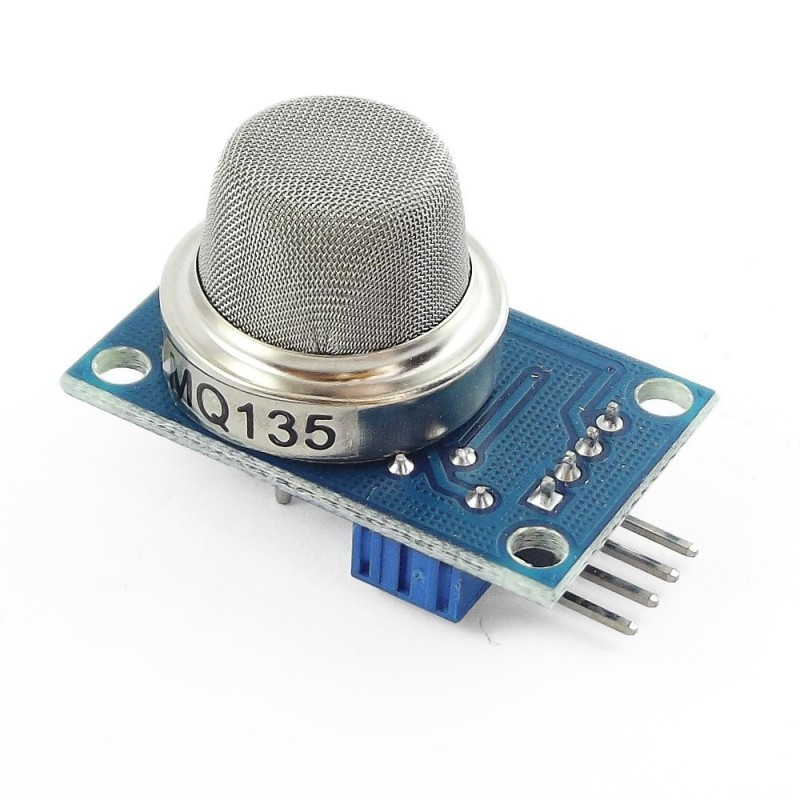
\includegraphics{aqi.jpg}\\
	
	The air quality sensor is also a MQ-135 sensor for detecting venomous gases that are present in the air in homes and offices. The gas sensor layer of the sensor unit is made up of tin dioxide (SnO2); it has lower conductivity compare to clean hair and due to air pollution the conductivity is increases. The air quality sensor detects ammonia, nitrogen oxide, smoke, CO2 and other harmful gases. The air quality sensor has a small potentiometer that permits the adjustment of the load resistance of the sensor circuit. The 5V power supply is used for air quality quality sensor.
	
	The air quality sensor is a signal output indicator instruction. It has two outputs: analog output and TTL output. The TTL output is low signal light which can be accessed through the IO ports on the Microcontroller. The analog output is an concentration, i.e. increasing voltage is directly proportional to increasing concentration. This sensor has a long life and reliable stability as well.\\
	
	\textbf{Content Applications Of MQ 135 Gas Sensor}
	
	The following are the applications of the MQ 135 gas sensor:
	
	•	Air quality monitor
	
	•	Detection of harmful gases
	
	•	Domestic air pollution detection
	
	•	Industrial pollution detection
	
	•	Portable air pollution detection\\\\
	
	\textbf{	Characteristics Of MQ-135}
	
	•	Good sensitivity to harmful gases in wide range.
	
	•	It has long life and low cost.
	
	•	Possesses high sensitivity to ammonia, benzene, sulfide gases.
	
	•	It is a simple drive circuit\\\\
	
	The MQ series of gas sensors use a small heater inside with an electro-chemical sensor. They are sensitive for a range of gases and are used indoors at room temperature.
	They can be calibrated more or less (see the section about "Load-resistor" and "Burn-in") but a know concentration of the measured gas or gases is needed for that.
	\\\\
	\textbf{Connections for the sensor}
	\\\\
	\textbf{Wiring}
	
	The preferred wiring is to connect both 'A' pins together and both 'B' pins together. It is safer and it is assumed that is has more reliable output results. Although many schematics and data-sheets show otherwise, you are advised to connect both 'A' pins together and connect both 'B' pins together.
	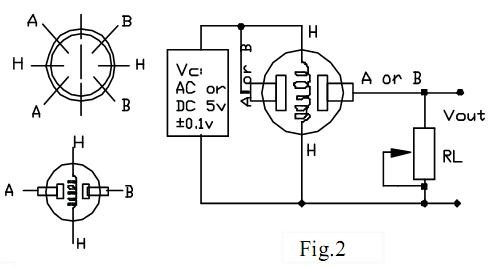
\includegraphics{mq135.jpg}
	In the picture, the heater is for +5V and is connected to both 'A' pins. This is only possible if the heater needs a fixed +5V voltage.
	The variable resistor in the picture is the load-resistor and it can be used to determine a good value. A fixed resistor for the load-resistor is used in most cases.
	The $V_{out}$ is connected to an analog input of the Arduino.
	\\\\
	\textbf{The heater}
	
	The voltage for the internal heater is very important.
	Some sensors use 5V for the heater, others need 2V. The 2V can be created with a PWM signal, using analogWrite() and a transistor or logic-level mosfet.
	The heater may not be connected directly to an output-pin of the Arduino, since it uses too much current for that.
	Some sensors need a few steps for the heater. This can be programmed with an analogWrite() function and delays. A transistor or logic-level mosfet should also in this situation be used for the heater.
	If it is used in a battery operated device, a transistor or logic-level mosfet could also be used to switch the heater on and off.
	The sensors that use 5V or 6V for the internal heater do get warm. They can easily get 50 or 60 degrees Celcius.
	After the "burn-in time", the heater needs to be on for about 3 minutes (tested with MQ-2) before the readings become stable.
	\\\\
	\textbf{Load-resistor}
	
	The sensor needs a load-resistor at the output to ground. It's value could be from $2kOhm$ to $47kOhm$. The lower the value, the less sensitive. The higher the value, the less accurate for higher concentrations of gas.
	If only one specific gas is measured, the load-resistor can be calibrated by applying a know concentration of that gas. If the sensor is used to measure any gas (like in a air quality detector) the load-resistor could be set for a value of about 1V output with clean air.
	Choosing a good value for the load-resistor is only valid after the burn-in time.
	\\\\
	\textbf{Burn-in}
	
	Some data-sheets use the term "preheat", but it is the time to burn-in the sensor. This is meant to make the sensor readings more consistent. A time of 12 or 24 hours is usually used for the burn-in time.
	The Burn-in is achieved by applying normal power to the sensor (to the heater and with the 'A' and 'B' pins connected, and with a load-resistor). In some special cases a specific burn-in is needed.
	\\\\
	
	\underline{{\LARGE \textbf{BMP 180} Pressure Sensor}}
	\\
	
	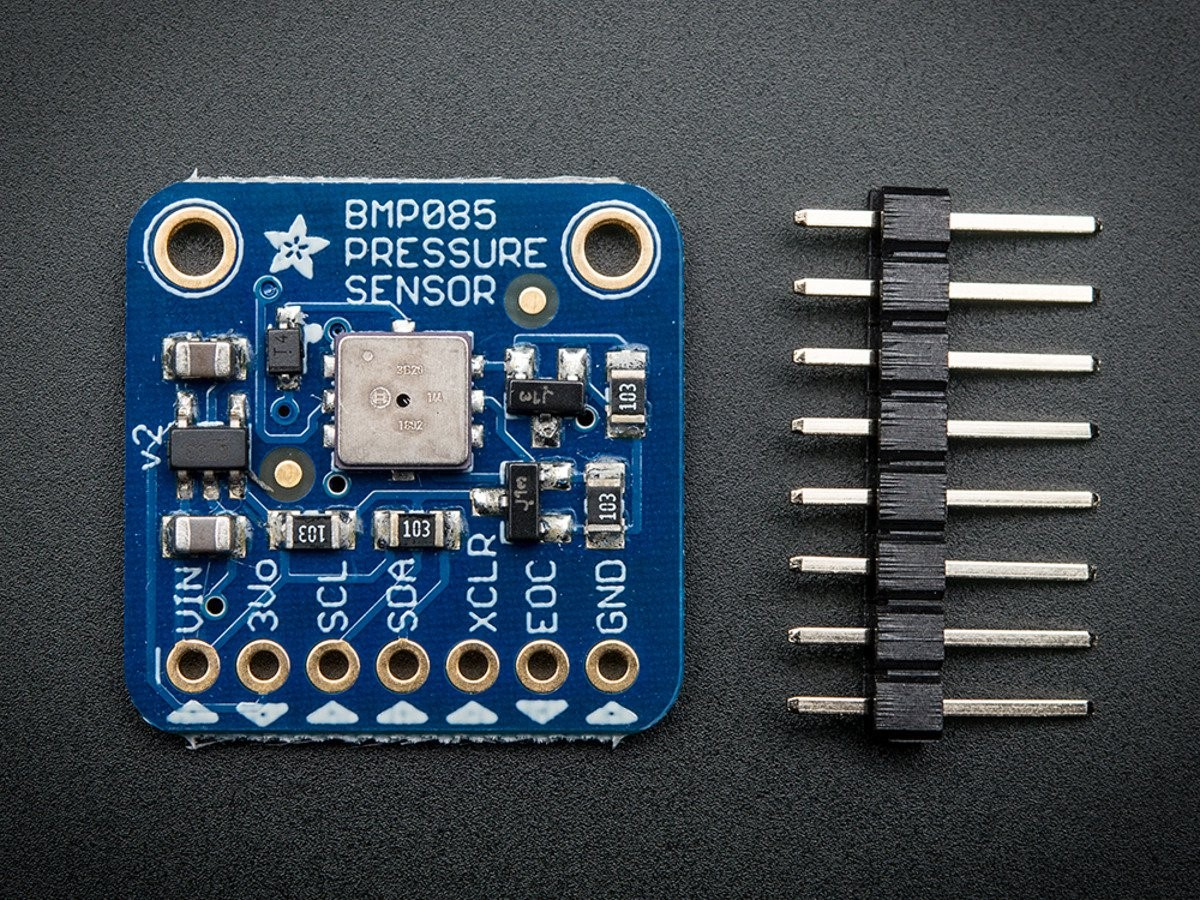
\includegraphics{bmp.jpg}\\
	
	 The BMP180 is the function compatible, new generation of high precision digital pressure sensors for consumer applications. The BMP180 is designed to be connected directly to a microcontroller of a mobile device via the I2C bus. The BMP180 consists of a piezo-resistive sensor, an analog to digital converter and a control unit with E2PROM and a serial I2C interface. It delivers the uncompensated value of pressure and temperature. The E2PROM has stored 176 bit of individual calibration data. This is used to compensate offset, temperature dependence and other parameters of the sensor. The BMP180 is based on piezo-resistive technology for EMC robustness, high accuracy and linearity as well as long term stability.
	 \\
	 
	 \textbf{Pin Configuration}\\
	 
	 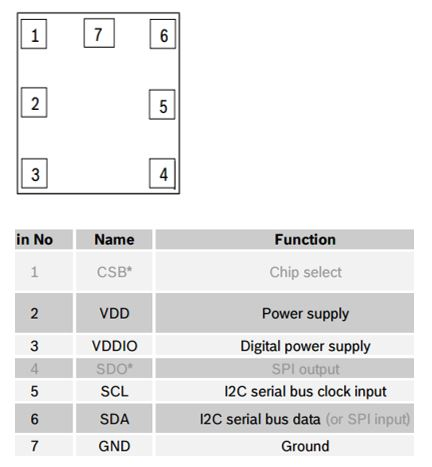
\includegraphics{pinbmp.jpg}
	 \\
	 
	 \textbf{Working}
	 
	 •	Calculation of true temperature and pressure in steps of 1Pa (= 0.01hPa = 0.01mbar) and temperature in steps of 0.1°C.
	 
	 •	With the measured pressure p and the pressure at sea level p0 e.g. 1013.25hPa, the altitude in meters can be calculated with the international barometric formula:
	 $$altitude = 44330*(1-P/P_{0})^{1/5.255}$$
	 •	With the measured pressure p and the absolute altitude the pressure at sea level can be calculated:
	 $$P_{0} = P/(1-altitude/44330)^{5.255}$$
	 
	\textbf{I2C Interface}
	
	 I 2C is a digital two wire interface  with clock frequencies up to 3.4Mbit/sec. (I2C standard, fast and high-speed mode supported) .SCL and SDA needs a pull-up resistor, typ. 4.7kOhm to VDDIO (one resistor each for all the I2C bus) The I2C bus is used to control the sensor, to read calibration data from theE2PROM and to read the measurement data when A/D conversion is finished. SDA (serial data) and SCL (serial clock) have open-drain outputs
	 \\
	 
	 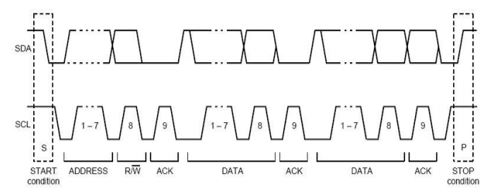
\includegraphics{I2C.jpg}
	 \\
	 
	 \textbf{\textbf{I2C protocol}} 
	 
	 The I2C interface protocol has special bus signal conditions. Start (S), stop (P) and binary data conditions are shown below. At start condition, SCL is high and SDA has a falling edge. Then the slave address is sent. After the 7 address bits, the direction control bit R/W selects the read or write operation. When a slave device recognizes that it is being addressed, it should acknowledge by pulling SDA low in the ninth SCL (ACK) cycle. At stop condition, SCL is also high, but SDA has a rising edge. Data must be held stable at SDA when SCL is high. Data can change value at SDA only when SCL is low. Even though VDDIO can be powered on before VDD, there is a chance of excessive power consumption (a few mA) if this sequence is used, and the state of the output pins is undefined so that the bus can be locked. Therefore, VDD must be powered before VDDIO unless the limitations above are understood and not critical.
	 \\
	 
	\textbf{Typical applications}
	\\
	 	 
	 •	Enhancement of GPS navigation (dead-reckoning, slope detection, etc.) 
	 
	 •	In- and out-door navigation 
	 
	 •	Leisure and sports
	 
	 •	Weather forecast 
	 
	 •	Vertical velocity indication (rise/sink speed)\\\\
	 
	 \underline{{\LARGE \textbf{LCD screen}}}\\
	 
	 LCD (Liquid Crystal Display) screen is an electronic display. A 16x2 LCD display is very basic module and is very commonly used in various devices and circuits. These modules are preferred over seven segments and other multi segment LEDs. The reasons being: LCDs are economical; easily programmable; have no limitation of displaying special and even custom characters (unlike in seven segments), animations and so on.
	 
	 A 16x2 LCD means it can display 16 characters per line and there are 2 such lines. In this LCD each character is displayed in 5x7 pixel matrix. This LCD has two registers, namely, Command and Data.
	 
	 The command register stores the command instructions given to the LCD. A command is an instruction given to LCD to do a predefined task like initializing it, clearing its screen, setting the cursor position, controlling display etc. The data register stores the data to be displayed on the LCD. The data is the ASCII value of the character to be displayed on the LCD. 
	 \\\\
	 \textbf{Pin Diagram}\\
	 
	 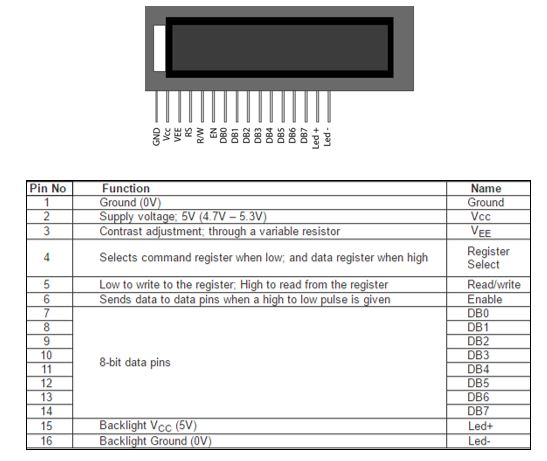
\includegraphics{lcd.jpg}\\
	 
	 
	  \underline{{\LARGE \textbf{DHT 11 sensor}}}\\
	  
	  The DHT11 is a basic, low-cost digital temperature and humidity sensor. It uses a capacitive humidity sensor and a thermistor to measure the surrounding air, and spits out a digital signal on the data pin (no analog input pins needed). Its fairly simple to use, but requires careful timing to grab data. The only real downside of this sensor is you can only get new data from it once every 2 seconds.
	  \\
	  
	  {\Large Features}
	  
	  	Full range temperature compensated
	  
	  	Relative humidity and temperature measurement
	  
	  	Calibrated digital signal
	  
	  	Outstanding long-term stability
	  
	  	Extra components not needed
	  
	  	Long transmission distance
	  
	  	Low power consumption
	  
	  	4 pins packaged and fully interchangeable
	  \\
	  
	  \textbf{Pin Configuration}\\
	  
	  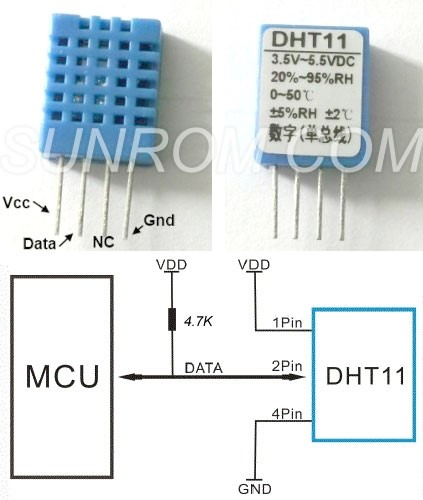
\includegraphics[width=10cm,height=10cm,keepaspectratio]{dht11.jpg}\\\\
	
	 
	 \textbf{Working}
	 \\
	 
	 1. Typical application circuit recommended in the short cable length of 20 meters on the 5.1K pull-up resistor, the resistance of greater than 20 meters under the pull-up resistor on the lower of the actual situation.
	 
	 2. When using a 3.5V voltage supply cable length shall not be greater than 20cm. Otherwise, the line voltage drop will cause the sensor power supply shortage, caused by measurement error.
	 
	 3. Each read out the temperature and humidity values are the results of the last measurement For real-time data, sequential read twice, but is not recommended to repeatedly read the sensors, each read sensor interval is greater than 5 seconds can be obtained accurate data.
	 
	 Communication Process: Serial Interface (Single-Wire Two-Way)
	 
	 The interesting thing in this module is the protocol that uses to transfer data. All the sensor readings are sent using a single wire bus which reduces the cost and extends the distance. In order to send data over a bus you have to describe the way the data will be transferred, so that transmitter and receiver can understand what says each other. This is what a protocol does. It describes the way the data are transmitted. On DHT-11 the 1-wire data bus is pulled up with a resistor to VCC. So if nothing is occurred the voltage on the bus is equal to VCC. Communication Format can be seperated into three stages
	 
	 1) Request
	 
	 2) Response
	 
	 3) Data Reading\\
	 
	 \textbf{Applications}
	 
	 1.	HVAC 
	 
	 2.	dehumidifier
	 
	 3.	testing and inspection equipment
	 
	 4.	consumer goods 
	 
	 5.	automotive, automatic control
	 
	 6.	data loggers
	 
	 7.	weather stations
	 
	 8.	home appliances 
	 
	 9.	humidity regulator
	 
	10. medical
	 
	 
	 \chapter*{\begin{center}
	 		SOFTWARE \\ REQUIREMENTS
	 	\end{center}}
	 	
	 \chapter*{\begin{center}
	 		Wunderground API
	 	\end{center}}
	 	
	 		
	 		Wunderground API is a weather forecast API provided by Weather.com. This can be used to get weather information of almost any major cities in the world. Wunderground delivers data as an HTTP response in a JSON file document.\\
	 		
	 		\textbf{Data Extraction}
	 		\\
	 		Data from the HTTP response is stored into a string and using Python's JSON library the string is broken into a Python dictionary for easy access of data.\\
	 		
	 		\textbf{HTTP Request and Response}
	 		\\
	 		To extract the data, the Python program first issues an HTTP request to the URL: 'http://api.wunderground.com/api/\textless Your API Key \textgreater /forecast/q/IN/Bangalore.json'
	 		\begin{verbatim}
	 		"period":1,
	 		"high": {
	 		"fahrenheit":"79",
	 		"celsius":"26"
	 		},
	 		"low": {
	 		"fahrenheit":"71",
	 		"celsius":"22"
	 		},
	 		"pop":80,
	 		"qpf_allday": {
	 		"in": 0.13,
	 		"mm": 3
	 		},
	 		"qpf_day": {
	 		"in": 0.06,
	 		"mm": 2
	 		},
	 		"qpf_night": {
	 		"in": 0.09,
	 		"mm": 2
	 		},
	 		"maxwind": {
	 		"mph": 10,
	 		"kph": 16,
	 		"dir": "SE",
	 		"degrees": 136
	 		},
	 		"avewind": {
	 		"mph": 5,
	 		"kph": 8,
	 		"dir": "SE",
	 		"degrees": 136
	 		},
	 		"avehumidity": 48,
	 		"maxhumidity": 0,
	 		"minhumidity": 0
	 		}
	 		},
	 		\end{verbatim}
	 		
	 		\textbf{HTTP}\\
	 		HTTP an acronym for Hyper Text Transfer Protocol. It defines the rules by which Internet traffic flows from one node to another. It comprises of two parts, HTTP request and HTTP response. HTTP request is the routine to access the webpage or webservice, while Response is the response sent back by the server to the client. The response can be either the html webpage or some requested data. It depends on the server script.\\
	 		
	 		\textbf{Data Curation}\\
	 		Selective data from the JSON file is taken out and packed into a local JSON file for further processing.
	\chapter*{\begin{center}
			REST API for python by twilio
		\end{center}}	
		
		Short Message Service (SMS) text messages are ubiquitous for communication all over the world. It is easy to send SMS text messages from a Python application using a web application programming interface (API). Let's take a look at the tools we need to quickly add SMS capability to our Python apps.
		
		For the above we require a rest api.
		\\
		
		\textbf{REST API}
		
		Representational state transfer (REST) or RESTful Web services are one way of providing interoperability between computer systems on the Internet. REST-compliant Web services allow requesting systems to access and manipulate textual representations of Web resources using a uniform and predefined set of stateless operations. Other forms of Web service exist, which expose their own arbitrary sets of operations such as WSDL and SOAP.[1] "Web resources" were first defined on the World Wide Web as documents or files identified by their URLs, but today they have a much more generic and abstract definition encompassing every thing or entity that can be identified, named, addressed or handled, in any way whatsoever, on the Web. In a RESTful Web service, requests made to a resource's URI will elicit a response that may be in XML, HTML, JSON or some other defined format. The response may confirm that some alteration has been made to the stored resource, and it may provide hypertext links to other related resources or collections of resources. Using HTTP, as is most common, the kind of operations available include those predefined by the HTTP verbs GET, POST, PUT, DELETE and so on. By making use of a stateless protocol and standard operations, REST systems aim for fast performance, reliability, and the ability to grow, by re-using components that can be managed and updated without affecting the system as a whole, even while it is running.
		\\
		
		\textbf{TWILIO}
		
		Twilio is a cloud communications platform as a service (PaaS) company based in San Francisco, California. Twilio allows software developers to programmatically make and receive phone calls and send and receive text messages using its web service APIs. Twilio's services are accessed over HTTP and are billed based on usage.
		
		Twilio uses Amazon Web Services to host telephony infrastructure and provide connectivity between HTTP and the public switched telephone network (PSTN) through its APIs.[20]
		
		Twilio follows a set of architectural design principles to protect against unexpected outages, and received praise for staying online during the widespread Amazon Web Services outage in April 2011.[21]
		
		Twilio supports the development of open-source software and regularly makes contributions to the open-source community. In June 2010 Twilio launched OpenVBX, an open-source product that lets business users configure phone numbers to receive and route phone calls.One month later, Twilio engineer Kyle Conroy released Stashboard, an open-source status dashboard written in the Python programming language that any API or software service can use to display whether their service is functioning properly.Twilio also sponsors Localtunnel, created by now ex-Twilio engineer Jeff Lindsay, which enables software developers to expose their local development environment to the public internet from behind a NAT.
		
		Twilio lists a number of other open-source projects on their website including:
		
		\textbf{Flask Restful}: Python Flask (web framework) to build REST APIs.
		
		\textbf{Shadow}: Runs requests through a release candidate with real production 
		
		traffic.
		
		\textbf{Banker’s Box}: Wrapper for storage backend.
		\\
		
		how to send sms can be found on \texttt{https://github.com/akhiljns/fluffy-codes}
		
	 		
	 		 	
	 		\chapter*{\begin{center}
	 		 		AdaFruit sensors libraries for python
	 		 	\end{center}}
	 		 
	 		 Many small embedded systems exist to collect data from sensors, analyse the data, and either take an appropriate action or send that sensor data to another system for processing.
	 		 
	 		 One of the many challenges of embedded systems design is the fact that parts you used today may be out of production tomorrow, or system requirements may change and you may need to choose a different sensor down the road.
	 		 
	 		 Creating new drivers is a relatively easy task, but integrating them into existing systems is both error prone and time consuming since sensors rarely use the exact same units of measurement.
	 		 
	 		 By reducing all data to a single sensors\_event\_t 'type' and settling on specific, standardised SI units for each sensor family the same sensor types return values that are comparable with any other similar sensor. This enables you to switch sensor models with very little impact on the rest of the system, which can help mitigate some of the risks and problems of sensor availability and code reuse.
	 		 
	 		 The unified sensor abstraction layer is also useful for data-logging and data-transmission since you only have one well-known type to log or transmit over the air or wire.		
	 		
	 		Therefore we have used Adafruit sensors libraries for following sensors:\\
	 		
	 		Adafruit\_MQ\-135(for Air quality index sensor)
	 		
	 		Adafruit\_DHT11(for temperature and humidity)
	 		
	 		Adafruit\_CharLCD(for lcd on raspberry pi)
	 		
	 		Adafruit\_BMP(for pressure and sea level)
	 		
	 		\chapter*{\begin{center}
	 				Expected Outcome
	 			\end{center}}
	 			
	 			We implemented a small weather station using raspberry pi. These small weather stations can be used by small scale farmers so that they can get weather information for their crops directly on their mobile devices
	 			
	 			it is an automated weather station which provides all kinds of information a farmer would require for their crop.
	 			
	 			The measurements taken by our weather station include temperature, atmospheric pressure, humidity, wind speed, wind direction,air quality index and precipitation amounts. Wind measurements are taken with as few other obstructions as possible, while temperature and humidity measurements are kept free from direct solar radiation, or insolation. Manual observations are taken at least once daily, while automated measurements are taken at least once an hour. Weather conditions out at sea are taken by ships and buoys, which measure slightly different meteorological quantities such as sea surface temperature (SST), wave height, and wave period
	 				
		\chapter*{\begin{center}
				Result 
			\end{center}}
			
			The result given by the python scripts is the main json file which store all the data collected from sensors , this data then is passed to the main shell scripts where it is called and the data is sent over sms on mobile phones every hour.
			
			This is the result which we are getting through sms.
			
			1. Temperature
			 
			2. Humidity
			
			3. Rainfall(Probablity of Precpitation) 
			
			4. Wind Direction
			
			5. Wind speed
			
			6. Pressure
			
			7. UV index
\end{document}